\documentclass[14pt]{extarticle}
\usepackage[left=3cm, right=3cm]{geometry}
\usepackage{amsmath, amssymb}
\usepackage{nccmath}
\usepackage{amsthm}
\usepackage{comment}
\usepackage{caption}
\usepackage{subcaption}
\usepackage{enumitem}
\usepackage{graphicx}
\usepackage[math]{cellspace}
    \cellspacetoplimit 4pt
    \cellspacebottomlimit 4pt
\usepackage{titletoc}
\usepackage{float}
\usepackage{imakeidx}
\usepackage{hyperref}
\newcolumntype{P}[1]{>{\centering\arraybackslash}p{#1}}
\hypersetup{
    colorlinks=true,
    linkcolor=black,
    urlcolor=blue,
    linktoc=all
}

\linespread{1.2}
\title{{\Huge Market Basket Analysis}\\{\Large Master in Data Science}}
\bigskip
\author{\bigskip \\ \bigskip{\Large Alberto Bertoncini 983833}\\ \smallskip{\Large Massimo Cavagna 983820}\\ \bigskip \href{https://github.com/Bertonc98/ProgettoAMD}{Github repository} }

\begin{document}
\maketitle
\newpage
\tableofcontents
\newpage
\section{Introduction}
The purpose of this paper is to present some of the techniques used in order to perform the so called "market/basket" analysis for a huge amount of data.
At first, these techniques were exploited for the analysis of purchases in markets, trying to find some relationships among goods bought by customers.
The idea is to try to discover associations between goods so that can be claimed that if a customer buy item (or a set of items) A he is also likely to buy item (or a set of items) B.
This relationship between A and B it is also called "association rule" and it is denoted as A $\rightarrow$ B.
Given A $\rightarrow$ B, in order to find out if it is a relevant association rule in a dataset some indexes must be taken into account:
\begin{itemize}[leftmargin=*]
	\vspace{-0.4cm}\item[-]{frequency/support}: the first requirement of an association rule to be considered "important" is the "high" frequency, so that can be observed that buying A and B together is something that occurs multiple times. An association rule is frequent if its frequency is above a given threshold.
	\vspace{-0.4cm}\item[-]{confidence}: given A $\rightarrow$ B, it states the probability that a customer buys B given that he bought A (P(B|A)). If an association rule is frequent and has high confidence it is called "strong".
	\vspace{-0.4cm}\item[-]{interest}: it tells if A and B are independent, directly or inversely correlated.
\end{itemize}
A general method that can be used to extract strong association rule is to find frequent itemsets and then to compute all the possible association rules between the subsets of each frequent itemset checking their confidence. Anyway, the focus of this paper will be entirely in showing how to extract frequent itemset from a large dataset.
In particular, three main algorithms will be implemented:
\vspace{-0.2cm}\begin{itemize}[leftmargin=*]
\item[-] A-priori:
\vspace{-0.4cm}\begin{itemize}
\item[-] base
\vspace{-0.2cm}\item[-] PCY
\end{itemize}
\vspace{-0.4cm}\item[-] SON
\vspace{-0.4cm}\item[-] Toivonen
\end{itemize}
\section{Dataset}
The dataset the dataset on which the analysis was carried out is the "\href{https://www.kaggle.com/ashirwadsangwan/imdb-dataset}{IMDb dataset}" (version 6). It is composed by data collected from the homonymous site IMDb. This dataset contains information about movies (long, short, tv series), their ratings and workers that have taken part in them. The data is divided into several files to simplify the analysis over specific aspect:
\begin{itemize}[leftmargin=*]
\vspace{-0.4cm}\item[-]{\it title.akas.tsv} contains informations about the localized version of the movies.
\vspace{-0.4cm}\item[-]{\it title.basics.tsv} contains general information about the movies, not influenced by the localization.
\vspace{-0.4cm}\item[-]{\it title.principals.tsv} contains information about the cast and the crew for each movie.
\vspace{-0.4cm}\item[-]{\it title.ratings.tsv} contains the IMDb rating informations about the movies.
\vspace{-1.0cm}\item[-]{\it name.basics.tsv} contains informations about the cast and the crew.
\end{itemize}
\section{Data structure}
{\it title.principal.tsv} is a tsv file with the subsequent structure:
\begin{itemize}[leftmargin=*]
\vspace{-0.4cm}\item[-]{\it tconst} (string) is an alphanumeric identifier of the movie.
\vspace{-0.4cm}\item[-]{\it ordering} (integer) is a number used to uniquely identify rows for a given movie.
\vspace{-0.4cm}\item[-]{\it nconst} (string) is an alphanumeric identifier of the cast/crew person.
\vspace{-0.4cm}\item[-]{\it category} (string) is the role of that person in the movie (a person can do different roles in the same movie). Possible values: 'actor', 'actress', 'archive footage', 'archive sound', 'cinematographer', 'composer', 'director', 'editor', 'producer', 'production designer', 'self', 'writer'.
\vspace{-0.4cm}\item[-]{\it job} (string) is a further specification of the role (can be empty, with the symbol "\textbackslash N").
\vspace{-0.4cm}\item[-]{\it characters} (string) is the name of the character played (can be empty, with the symbol"\textbackslash N").
\end{itemize}
There are 36.499.704 rows for 5.710.740 different movies.\\
Only rows with an actor are considered, so the analysis is done over 14.830.233 rows.\\
Movies without any registered actor need to be filtered, reducing the number of movies to 3.602.200.\\
In the end the number of different actors in this dataset is 1.868.056.\\
The size of {\it title.principal.tsv} is 1.6 GB.\\

\noindent
{\it name.basics.tsv} isa  tsv file with the subsequent structure:
\begin{itemize}[leftmargin=*]
\vspace{-0.4cm}\item[-]{\it nconst } (string) is an alphanumeric identifier of the cast/crew person.
\vspace{-1.1cm}\item[-]{\it primaryName } (string) the name of the person.
\vspace{-0.4cm}\item[-]{\it birthYear } (YYYY) year of birth.
\vspace{-0.4cm}\item[-]{\it deathYear  } (YYYY) year of death.
\vspace{-0.4cm}\item[-]{\it primaryProfession } (array of strings) the top 3 profession of the person.
\vspace{-1.0cm}\item[-]{\it knownForTitles  } (array of tconst) movies the person is known for (can be empty).
\end{itemize}
There are 9.711.022 rows in this file with only 3.625.895 people marked as actor/actress.
\\
\\
All the algorithms listed above will work analyzing sets of actors, so for each movie
will be defined an set of actors that worked in it.
Because of this, only a few datasets will be used: in particular {\it title.principal.tsv} from which is possible create sets of actors from each movie and {\it name.basics.tsv} from which is possible retrieve the names of the actors from their IDs.

\section{Preprocessing}
Before starting with the description and the implementation of the algorithms
data must be preprocessed in order to make them in a suitable form.\\
As already said, one of the main dataset used is the {\it title.principals.tsv}, since it contains all the information needed: the main idea in this phase is to group all the rows by the {\it tconst} (movie id), and take all the {\it nconst} that refers to an actor ({\it category}). Once this operation is performed, the resulting data are organized in sets (or baskets) of actors' IDs (one for each movie), so the next step is checking if all the baskets respect the "set shape" by deleting all the replicated IDs inside each basket.\\ 
The sets/baskets of IDs are groups of string values, so just for saving space purpose
the only action left is to change them with an integer: all the IDs are in the form of "nm" followed by a number, so it is rather easy to change them just cutting the first part.\\
In the end the completely transformed data are saved on secondary storage.\\

\section{Algorithms applied}
In this section are presented the algorithms used with the aim of obtaining the list of frequent itemsets (sets of actors in our case).\\
But first it is important to explain the property the algorithms are based on the anti-monotonicity property says that if a set is not frequent then all the its superset are not frequent. This property is fundamental since it allows to discard all the non-frequent sets from the analysis and so reducing the magnitude of computation.\\
Another fact to point out before starting with the description of the algorithms is that they are designed in order to work with a huge amount of data (big enough that can not fit in memory), so for all of them will be given particular attention to the number of mass memory access performed, which makes them slower.
\subsection{A-priori}
The first approach implemented is the basic A-priori algorithm. This algorithm can be outlined by two phases:
\begin{itemize}[leftmargin=*]
	\vspace{-0.4cm}\item[-] Construction: in this phase all the sets of dimension k are built from the frequent ones of dimension k-1. For implementation purposes, it will be shown that this phase contains a sorting pre-phase in which all the sets of dimension k-1 are sorted.
	\vspace{-0.4cm}\item[-] Filtering: in this phase all the new (candidate frequent ) sets obtained are filtered by their frequency, so that if they do not reach a given threshold they are discarded (according to the antimonotonicity property).
\end{itemize}
At the very first step the algorithm starts counting the number of occurrences of each item in the dataset (singleton), so in this phase the main memory is partially filled and the first scan of the data is performed. Once all the frequencies are found, the singletons are filtered using a predefined threshold.\\
Now, the algorithm scans again the dataset and for each basket builds a list of all the combinations of dimension 2 with items contained, not counting the frequency for the pairs composed by non frequent singletons. Again, the filtering step is performed.\\
From this point, the algorithm looks for all the tuples of dimension k $>$ 2 and it becomes important the sorting pre-phase mentioned before: in order to avoid duplications all the frequent tuples of dimension k-1 are "joined" if they have in common the first k-2 elements, then all the possible tuples of dimension k are built so that it is possible to check if a tuple is present or not in that basket.\\
These steps continue until it is not possible to find a single tuple of dimension k that is frequent.\\
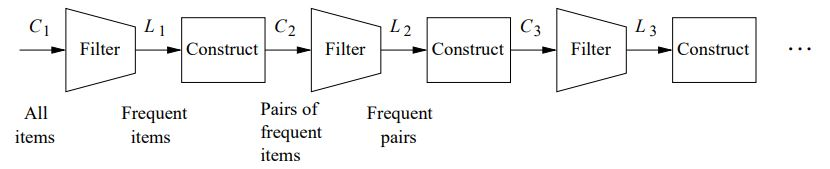
\includegraphics[scale=0.53]{apriori.jpg}

\subsection{PCY (single hash)}
An improvement of this algorithm is the PCY (Park, Chen, Yu) that exploit the memory's free space while counting the frequency of itemsets of given size k:
as the base apriori algorithm does, the first step is the counting of singleton frequency, but in this step, for each basket also all the pairs of items are computed
and with the use of an hash function they are mapped into a position in an hashmap and the corresponding position is updated incrementing the value by one. Once the baskets are fully scanned the hashmap is compressed into a bitmap, substituting with a 1 all those positions whose frequencies are above a threshold, 0 otherwise.
Of course the use of hash functions brings "collisions" so it is not sure that what a given hashmap position contains is the frequency of a single pair, but it is sure that if a frequency is not above the threshold all the pairs mapped in that position are not frequent.\\
At the next step, the pairs' frequencies are computed but only if the corrisponding bit in the bitmap is a 1 the frequency counter is created.\\
The same process is reapeted between pairs and triples and so on.
This version of the apriori algorithm allows to reduce significantly the number of sets kept in memory at each step, using the same number of access in the secondary storage of the basic apriori algorithm.\\
 
\subsection{SON}
This algorithm is designed with the purpose of parallelizing the computation of frequent itemsets, working over chunks (partition) of the data.\\
The idea is to exploit the basic apriori and the PCY algorithm but in a distributed manner so to reduce the computational workload:\\
The algorithm starts applying the Apriori or PCY on a single chunk, using as threshold for each chunk p*s, where p is the fraction of total baskets contained in a single chunck (so 1/p is the number of chunks), then all the results obtained are putted together and all the dataset is fully scanned in order to delete false positive, since a chunck can find a set whose support in bigger then p*s, but the sum of the frequencies coming from all the chunks is below s.


\subsection{Toivonen}
This algorithm exploits the Apriori or PCY algorithm, as the previous one, but it considers only a sample of data instead of chunks: 
the algorithm start by selecting a fraction p of all the baskets and adjusting the threshold s by multiplying q*p*s, where q is a integer very close to one (tipically 0.95). It continues by applying the basic apriori or the pcy to the sample and obtains the frequent sets in the sample. Now, the particularity of this algorithm is applied: the "negative border" is built by using a the sample's frequent sets.\\
The negative border is a set of itemsets that are not frequent, but whose immediate subset are frequent in the sample.\\
The last part is checking if there is a set in the negative border that is frequent in all the baskets: if there are no frequent sets, the algorithms outputs the frequent sets found in the sample, otherwise does not output anothing and the algorithm must bu re-runned with another sample.\\

\section{Implementation}
In this section will be presented some key points about the implementation of the agorithms described.\\
All the algorithms have been implemented from scratch in Python using some libraries only for computation purposes or the use of pre-built data structures.\\
SPARK IMPLEMENTATION?
\subsection{Preprocessing}
In the preprocessing phase the aim is to transform the data and reorganize them in a suitable way for the algorithms to be taken in input: as already mentioned in the "Preprocessing" section, one of the two main dataset used is "{\it title.principal.tsv}" from which all the baskets are built. This file is a .tsv file so it is easily readable with {\it read csv()} of CSV library. Because of the size of the file, the file is readed in chunks.\\
A chunk of data it is organized in a DataFrame as:\\
const (string) $|$ ordering (integer) $|$ nconst (string) $|$ category (string) $|$ job (string) $|$ characters (string)\\
so the first operation is filtering by the {\it category} selecting only {\it actor} or {\it actress} values. Then follows a "group-by" operation (using a the DataFrame.groupby method) over the {\it tconst} attribute. Each group is finally written in a the "basket.txt" file selecting only the {\it nconst} attribute and changing all the values from string to integers, removing possible duplicates.
This is an example of row contained in the output file:\\
2350007,525907,1151424,2354154\\

\subsection{A-priori}
Starting from the "basket.txt", the algorithm takes in input the iterator of the file and the support threshold. Reading row by row, it uses a list in order to save the singletons frequency, indexing each position with the id of the singleton itself. Once all the baskets are scanned, it filters out all the singleton whose support is below the threshold.\\
The algorithm now starts a loop in which it search for frequent sets of greater dimensions and stops only if it does not find any frequent set in a given dimension:
the first step in the loop is building all the tuples of dimension k starting from the frequent ones of dimension k-1. In order to avoid duplicates all the frequent sets are ordered in a increasing manner and a new set of dimension k is formed by the "join" of two other sets only if the latters have the first k-2 items in common.
For example, considering a two set of triples {1,2,3}, {1,2,4} it is possible to obtain a new set {1,2,3,4}.
All the resulting sets are saved in a Dictionary used to count their frequency. This operation is again performed by scanning all the baskets in the dataset and updating the frequency of the sets of dimension k, ignoring all those that contains a non frequent subset (antimonotonicity property). The dictionary is filtered by removing all the non frequent sets and its keys are saved in a list that store all the frequent sets found.
 
\subsection{PCY}
This algorithm uses the same data structure and performs the same steps as the previous one, but in addition works with an hashmap and a bitmap (as already explained in the section {\it PCY}): the implementation of the hashmap is done buy using the pre-built Python's "hash" function and a list. In the frequency updating phase of the itemset of length k, for each basket read from the file, all the combination of length k+1 are mapped in tha list updating the frequency counter.
To compress the hashmap in a bitmap is used the library Bitmap and it is created of the same length of the hashmap setting to one only those position whose value is greater the the threshold. Once all the bits are setted the hashmap is deleted.

\subsection{SON}
The SON algorithm has been implemented in order to compute with both the algorithms explained above. The main implementation difference is that the "basket.txt" file is divided in chunks and the basic Apriori/PCY is applied to a small set. The execution can be done in a serial or parallelized way, in this case the execution is performed sequentially. In the serial version, it takes in input the size of the chunk and reads only those number of rows at the time, then execute the chosen algorithm and saves the relulting frequent sets of each chunk in a list. When all the chunks have been analyzed, it is necessary to check the presence of FP: from the list of candidate frequent sets it is created a Dictionary and the full file is scanned again updating the frequency of the candidates; at the end, the Dictionary is filtered by frequency and all the true frequent sets are returned.

\subsection{Toivonen}
As the previous one, also this algorithm works with both the basic Apriori and the PCY and, since it is a merely application of one of the two over a sample of the dataset, the most relevant part is how the negative border is built: it starts taking all the non-frequent singletons from the sample, then for each k finds all the itemset of lenght k composed by frequent sets of length k-1 that are not frequent. This procedure in repeated for all k <= max(len(x)| x $\in$ {frequent candidate})+1. All the sets found are added to a list that will be converted into a Dictionary, as all the frequent candidates found by the Apriori/PCY. This two structure are particularly useful in subsequent step, that is search for false positive in the candidates and frequent itemset in the negative border, both considering the whole dataset: so the Dictionary will contain as key the itemset and as value its frequency.
At the end, if the NB contains itemset with frequency above the threshold the algorithm ends printing "no answer", otherwise it returns the frequent sets, previously filtered from false positive.

\section{Scaling of proposed solutions}
\section{Experiments}
\subsection{Size of candidates and timing with different algorithms}
In the following table are listed the execution time (last row) and the number of candidates generated for each size, considering the whole dataset.
\begin{center}
\begin{tabular}{ |c|c|c|c|c| } 
 \hline
 Size & Apriori & PCY & SON apriori & SON PCY \\
 \hline
 2 & 11144462 & 11144462 & 1311498 & 6880\\ 
 3 & 10011 & 33 & 2782 & 1866\\ 
 4 & 13 & 13 & 1297 & 1167\\ 
 5 & 2 & 2 & 737 & 690 \\
 6 & - & - & 374 & 358 \\
 7 & - & - & 136 & 133 \\
 8 & - & - & 30 & 30 \\
 9 & - & - & 3 & 3 \\
 10 & - & - & - & - \\
 \hline
 Sec & 87 & 335 & 292 & 584\\
 \hline
\end{tabular}
\end{center}
The number of candidates is the number of itemets of size k analyzed, created from the previous frequent itemsets of size k-1. The number of singletons is not reported since they are equal for all the algorithm.\\
In the first pair of columns is evident the improvement given by the PCY in filtering candidates, but, on the other hand, it is evident the PCY's computation time is nearly 4 times the Apriori's one. The same time difference is evident in the two SON algorithms.\\


\subsection{Size of candidates and times with different hash size (PCY)}
The subsequent chart shows the number of candidates found by the PCY algorithm with different hashmap sizes. It is evident that the increase of the hashmap size the number of candidates is lowered very quickly due to the decreasing probability of collisions.\\
The sequent measures are performed over the same sample, containing 600000 baskets, the algorithms has been completed in the times reported in the table.\\
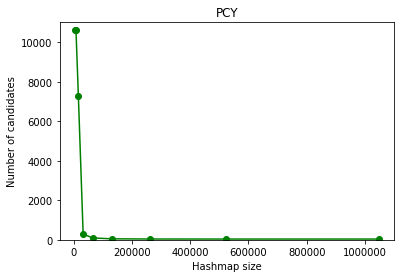
\includegraphics[scale=1]{size_by_hsize.png}\\
\begin{center}
\begin{tabular}{ |c||c|c|c|c|c|c|c|c|c| } 
 \hline
 Hash size & $2^{12}$ & $2^{13}$ & $2^{14}$ & $2^{15}$ & $2^{16}$ & $2^{17}$ & $2^{18}$ & $2^{19}$ & $2^{20}$ \\
 \hline
 Candidates & 10603 & 10603 & 7266 & 292 & 93 & 50 & 40 & 38 & 38\\
 \hline
\end{tabular}
\end{center}
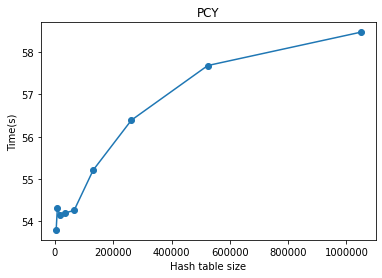
\includegraphics[scale=1]{pcy_hsize_time.png}\\
Regarding time, it can be seen an increment of computing times due to the handling of the hashmap, although it is just a difference of few seconds.\\
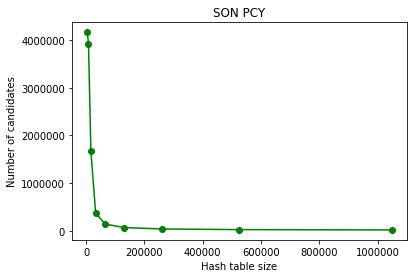
\includegraphics[scale=1]{sonpcy_candidates.png}\\
\begin{center}
\hspace*{-1,5cm}
\begin{tabular}{ |c||c|c|c|c|c|c|c|c|c| } 
 \hline
 Hash size & $2^{12}$ & $2^{13}$ & $2^{14}$ & $2^{15}$ & $2^{16}$ & $2^{17}$ & $2^{18}$ & $2^{19}$ & $2^{20}$ \\
 \hline
 Candidates & 1304840 & 1191355 & 432588 & 141776 & 59356 & 29983 &  4761 & 3438 & 2775 \\
 \hline
\end{tabular}
\end{center}
\subsection{Time at change of threshold}
This chart and table show the time of execution of each algorithm varying the threshold. 
The sequent measures are performed over the same sample, containing 600000 baskets.
It is important to underline that for the SON application (with both Apriori and PCY) only the worst time over a node has been saved due to the parallelized computation.\\

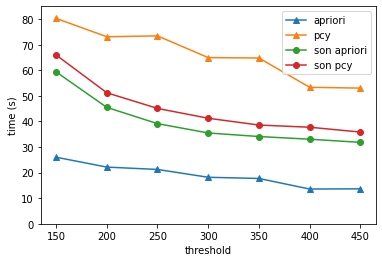
\includegraphics[scale=1.1]{times.png}\\
\begin{center}
\begin{tabular}{ |P{3cm}|P{2cm}|P{2cm}|P{2cm}|P{2cm}| } 
 \hline
 Threshold & Apriori & PCY & SON Apriori & SON PCY \\
 \hline
 150 & 26.04s & 80.30s & 59.40s & 66.00s\\
 200 & 22.17s & 73.13s & 45.51s & 51.23s\\
 250 & 21.24s & 73.46s & 39.15s & 45.10s\\
 300 & 18.19s & 64.96s & 35.51s & 41.26s\\
 350 & 17.72s & 64.81s & 34.12s & 38.60s\\
 400 & 13.59s & 53.35s & 33.07s & 37.75s\\
 450 & 13.67s & 53.04s & 31.83s & 35.86s\\
 \hline
\end{tabular}
\end{center}
\subsection{Size of negative border}
Concerning the Toivonen algorithm the key point is the analysis of the Negative border, because the extraction of frequent candidates is only an application of one of the Apriori or PCY algorithm.\\
In the following figure it is shown the negative border size variation changing the threshold using a sample of 600367 (1/6 of the total dataset): the increasing of the threshold produce a lower number of candidates and so a smaller negative border.\\
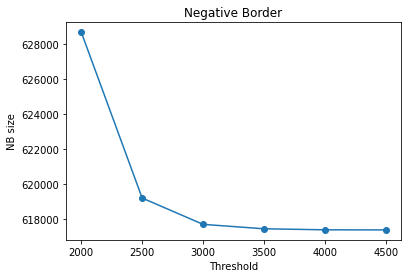
\includegraphics[scale=1]{nb_sizes.png}\\
\section{Results}
{\it I/We declare that this material, which I/We now submit for assessment, is entirely my/our own work and has not been taken from the work of others, save and to the extent that such work has been cited and acknowledged within the text of my/our work. I/We understand that plagiarism, collusion, and copying are grave and serious offences in the university and accept the penalties that would be imposed should I engage in plagiarism, collusion or copying. This assignment, or any part of it, has not been previously submitted by me/us or any other person for assessment on this or any other course of study.}

\begin{comment}
The report should contain the following information:

-the chosen dataset, and the parts of the latter which have been considered,
-how data have been organized,
-the applied pre-processing techniques,
-the considered algorithms and their implementations,
-how the proposed solution scales up with data size,
-a description of the experiments,
-comments and discussion on the experimental results.

\end{comment}
\end{document}

